\section*{سوال ۵}

در این بخش، پنج مفهوم مدل‌سازی عمده در مهندسی نرم‌افزار -
\lr{DFD}
،
\lr{UML}
،
\lr{User Story}
،
\lr{CRC Card}
و
\lr{BPMN}
- مورد بررسی و مقایسه قرار دهید از جنبه‌های مختلف.

\begin{itemize}
	\item چه چیزهایی را مدل می‌کنند
	\item آن‌ها را چگونه مدل می‌کنند
	\item کجا/در چه زمانی استفاده می‌شوند
	\item تفاوت سطح انتزاع در مدل‌سازی
\end{itemize}

\section*{جواب سوال ۵}

در مهندسی نرم‌افزار، مدل‌سازی فرایندی است که به منظور ایجاد یک نمایش گرافیکی یا نمادین از یک سیستم، فرایند یا مفهوم انجام می‌شود. مدل‌سازی می‌تواند برای اهداف مختلفی استفاده شود، از جمله:

تجسم سیستم یا فرآیند

درک بهتر سیستم یا فرآیند

ارتباط موثرتر با سایرین در مورد سیستم یا فرآیند

تجزیه و تحلیل و بهبود سیستم یا فرآیند

در این مقاله، مفاهیم مختلف مدل‌سازی در مهندسی نرم‌افزار را تحلیل و مقایسه می‌کنیم.

\section*{\lr{DFD (Data Flow Diagram)}}
DFD ، که مخفف \lr{Data Flow Diagram} است، یک ابزار مهم در مهندسی نرم‌افزار برای نمایش جریان داده‌ها درون یک سیستم است. این نمودار به تحلیل‌گران و طراحان کمک می‌کند تا درک عمیق‌تری از سیستم‌ها داشته باشند.

\begin{itemize}
	\item \textbf{کاربرد:} DFD برای نمایش جریان داده‌ها بین فرآیندها، داده‌ها، سازمان‌ها و ذخیره‌سازی‌ها در سیستم‌های نرم‌افزاری استفاده می‌شود.
	\item \textbf{ساختار:} DFD شامل گره‌ها و خطوط است. گره‌ها نشان‌دهنده فرآیندها، مخازن داده، منابع داده و مقاصد داده هستند، و خطوط جریان داده‌ها را نشان می‌دهند.
	\item \textbf{سطح انتزاع:} DFD در سطوح مختلف انتزاع مورد استفاده قرار می‌گیرد.
	\item \textbf{مزایا:} این ابزار به شناسایی مسیرهای داده و تحلیل چگونگی انجام کار توسط سیستم کمک می‌کند.
\end{itemize}

\begin{figure}[H]
	\centering
	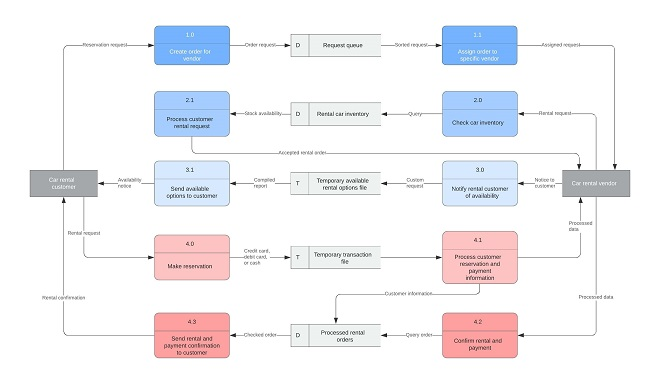
\includegraphics{pic8.png}
	\label{fig:label4}
\end{figure}

\subsection*{\lr{UML (Unified Modeling Language)}}
UML ، که مخفف \lr{Unified Modeling Language} است، یک زبان استاندارد برای مدل‌سازی و توصیف ساختار و رفتار سیستم‌های نرم‌افزاری است. این زبان از طریق استفاده از مجموعه‌ای متنوع از نمودارها کاربرد دارد.

\begin{itemize}
	\item \textbf{انتزاع در UML :} یکی از ویژگی‌های برجسته UML توانایی آن در نمایش سطوح مختلف انتزاع است.
	\item \textbf{کاربرد UML :} UML در تمام مراحل توسعه نرم‌افزار مورد استفاده قرار می‌گیرد.
\end{itemize}

\begin{figure}[H]
	\centering
	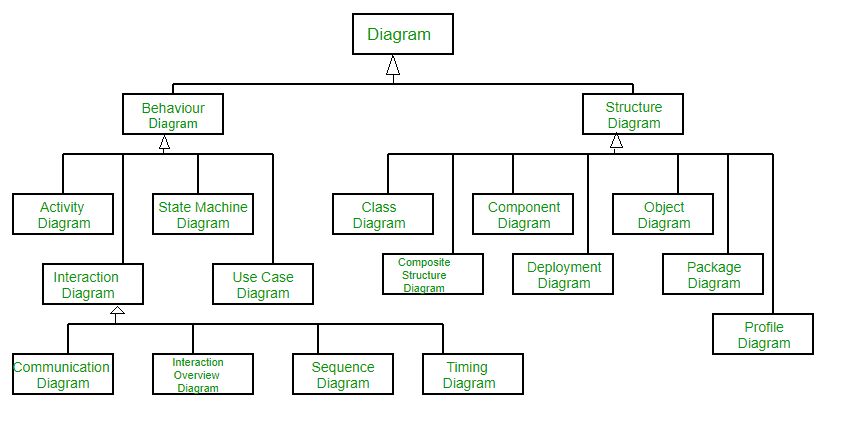
\includegraphics{pic9.png}
	\label{fig:label4}
\end{figure}

\subsection*{\lr{User Story}}
\lr{User Story} در مهندسی نرم‌افزار به عنوان یک تکنیک مدل‌سازی برای تعریف نیازمندی‌ها و رفتار کاربران در سیستم استفاده می‌شود. این روش متمرکز بر بیان خواسته‌ها و نیازهای کاربران از طریق سناریوهای کوتاه و روشن است.

\begin{itemize}
	\item \textbf{سطح انتزاع:} \lr{User Story} نسبت به سایر روش‌های مدل‌سازی، از سطح انتزاع بالاتری برخوردار است.
	\item \textbf{بررسی نیازمندی‌ها:} این روش نیازمندی‌ها را از دیدگاه ذی‌نفعان بررسی می‌کند.
	\item \textbf{مثال‌ها:} در سامانه دانشگاهی، 
	\lr{User Story}
	ها می‌توانند شامل مواردی مانند «من به عنوان یک دانشجو می‌خواهم لیست تمرین‌ها و ددلاین‌های آن‌ها را داشته باشم...» باشند.
\end{itemize}

\begin{figure}[H]
	\centering
	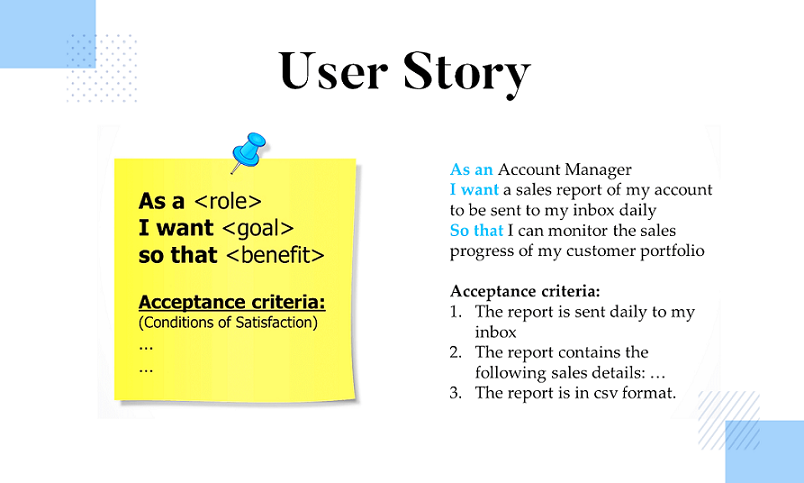
\includegraphics{pic7.png}
	\label{fig:label4}
\end{figure}

\subsection*{\lr{CRC Card}}

\lr{CRC Card} ، مخفف Class-Responsibility-Collaboration ، یک ابزار مدل‌سازی در مهندسی نرم‌افزار است که برای تحلیل و طراحی سیستم‌های شی‌گرا استفاده می‌شود. هر کارت CRC سه جزء اصلی دارد: کلاس، مسئولیت‌ها و همکاری‌ها.

\begin{itemize}
	\item \textbf{کلاس:} نام کلاس در بالای کارت قرار می‌گیرد و نشان‌دهنده یک مفهوم، شیء یا موجودیت در سیستم است.
	\item \textbf{مسئولیت‌ها:} این بخش شامل لیستی از وظایف یا مسئولیت‌هایی است که کلاس باید انجام دهد. این مسئولیت‌ها معمولاً عملیات یا رفتارهایی هستند که کلاس بر عهده دارد.
	\item \textbf{همکاری‌ها:} این بخش شامل کلاس‌های دیگری است که کلاس برای انجام مسئولیت‌های خود با آن‌ها همکاری می‌کند.
\end{itemize}

کارت‌های CRC به تیم‌های توسعه کمک می‌کنند تا ساختار کلاس‌های سیستم را درک کنند و نحوه تعامل آن‌ها با یکدیگر را تجزیه و تحلیل نمایند. این رویکرد تمرکز بر روی همکاری و مسئولیت‌های متقابل را ترویج می‌کند و به شناسایی و حذف وابستگی‌های غیرضروری کمک می‌کند.

\begin{figure}[H]
	\centering
	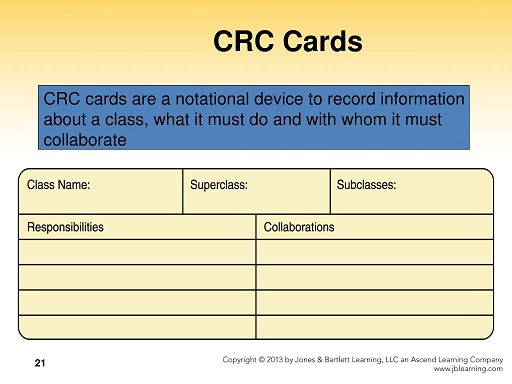
\includegraphics{pic6.jpg}
	\label{fig:label4}
\end{figure}

\subsection*{BPMN}

BPMN مخفف \lr{Business Process Model and Notation} به معنای مدل و نشانه‌گذاری فرآیند کسب‌وکار است. این یک زبان مدل‌سازی بصری برای برنامه‌های تجزیه و تحلیل کسب‌وکار و مشخص کردن گردش کار فرایندهای سازمانی است. BPMN توسط ابتکار مدیریت فرآیند کسب‌وکار (BPMI) توسعه یافت و از زمان ادغام دو سازمان در سال ۲۰۰۵ توسط گروه مدیریت اشیاء (OMG) حفظ شده ‌است.

\subsubsection*{عناصر اصلی}

BPMN از مجموعه‌ای از عناصر بصری برای مدل‌سازی فرآیندهای کسب‌وکار استفاده می‌کند. این عناصر عبارتند از:

\begin{itemize}
	\item فعالیت‌ها (Activities) : فعالیت‌ها اقداماتی هستند که در یک فرآیند انجام می‌شوند. فعالیت‌ها می‌توانند شامل کارهای فیزیکی، پردازش اطلاعات یا تصمیم‌گیری باشند.
	\item جریان‌ها (Flows) : جریان‌ها نحوه ارتباط فعالیت‌ها را نشان می‌دهند. جریان‌ها می‌توانند به صورت خط مستقیم، خط نقطه‌چین یا خط مورب نشان داده شوند.
	\item شروع و پایان \lr{(Start and End)} : شروع و پایان نشان‌دهنده نقاط شروع و پایان یک فرآیند هستند.
	\item کنترل‌ها (Controls) : کنترل‌ها شرایطی را که بر جریان فرآیند تأثیر می‌گذارند، نشان می‌دهند.
	\item پیوندها (Links) : پیوندها فعالیت‌ها یا جریان‌های مختلف را به هم متصل می‌کنند.
\end{itemize}

\subsubsection*{کاربردهای BPMN}

BPMN در طیف گسترده‌ای از کاربردها استفاده می‌شود، از جمله:

\begin{itemize}
	\item تجزیه و تحلیل فرآیندهای کسب‌وکار: BPMN می‌تواند برای تجزیه و تحلیل فرآیندهای کسب‌وکار موجود و شناسایی فرصت‌های بهبود استفاده شود.
	\item طراحی فرآیندهای کسب‌وکار جدید: BPMN می‌تواند برای طراحی فرآیندهای کسب‌وکار جدید استفاده شود.
	\item پیاده‌سازی فرآیندهای کسب‌وکار: BPMN می‌تواند برای پیاده‌سازی فرآیندهای کسب‌وکار در سیستم‌های فناوری اطلاعات استفاده شود.
	\item آموزش فرآیندهای کسب‌وکار: BPMN می‌تواند برای آموزش کارکنان در مورد فرآیندهای کسب‌وکار استفاده شود.
\end{itemize}

\subsubsection*{آینده BPMN}

BPMN یک زبان قدرتمند و انعطاف‌پذیر است که به سازمان‌ها کمک می‌کند تا فرآیندهای کسب‌وکار خود را به‌طور موثرتر مدیریت کنند. انتظار می‌رود که BPMN در سال‌های آینده به محبوبیت خود ادامه دهد، زیرا سازمان‌ها به دنبال راه‌هایی برای بهبود کارایی و بهره‌وری خود هستند.


\begin{figure}[H]
	\centering
	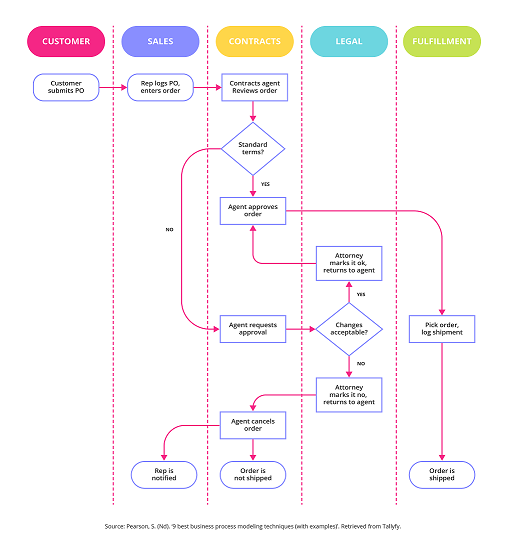
\includegraphics{pic5.png}
	\label{fig:label4}
\end{figure}




\subsection*{\lr{DFD (Data Flow Diagram)}}
\begin{itemize}
	\item \textbf{چه چیزهایی را مدل می‌کند:} جریان داده‌ها و ارتباطات بین فرایندها، داده‌ها و ذخیره‌سازی‌ها.
	\item \textbf{چگونگی مدل‌سازی:} با استفاده از نمودارهای گرافیکی برای نشان دادن جریان داده‌ها.
	\item \textbf{زمان استفاده:} در مراحل اولیه تحلیل سیستم برای درک بهتر جریان اطلاعات.
	\item \textbf{سطح انتزاع:} سطح بالا در ارتباط با جریان داده‌ها.
\end{itemize}

\subsection*{\lr{UML (Unified Modeling Language)}}
\begin{itemize}
	\item \textbf{چه چیزهایی را مدل می‌کند:} ساختار و رفتار سیستم‌های نرم‌افزاری.
	\item \textbf{چگونگی مدل‌سازی:} با استفاده از مجموعه‌ای متنوع از نمودارها (مانند نمودار کلاس، نمودار توالی).
	\item \textbf{زمان استفاده:} در تمام مراحل توسعه نرم‌افزار.
	\item \textbf{سطح انتزاع:} متغیر، بسته به نوع نمودار.
\end{itemize}

\subsection*{\lr{User Story}}
\begin{itemize}
	\item \textbf{چه چیزهایی را مدل می‌کند:} نیازمندی‌ها و ویژگی‌های کاربران از دیدگاه آن‌ها.
	\item \textbf{چگونگی مدل‌سازی:} به صورت جملات ساده و قابل فهم برای توصیف داستان‌های کاربری.
	\item \textbf{زمان استفاده:} بیشتر در رویکردهای توسعه چابک.
	\item \textbf{سطح انتزاع:} بسیار بالا و کاربر محور.
\end{itemize}

\subsection*{\lr{CRC Card (Class-Responsibility-Collaboration)}}
\begin{itemize}
	\item \textbf{چه چیزهایی را مدل می‌کند:} وظایف، مسئولیت‌ها و همکاری‌های کلاس‌ها.
	\item \textbf{چگونگی مدل‌سازی:} با استفاده از کارت‌هایی که کلاس‌ها و وظایف آن‌ها را نمایش می‌دهند.
	\item \textbf{زمان استفاده:} در مرحله طراحی سیستم و تعریف مسئولیت‌های کلاس‌ها.
	\item \textbf{سطح انتزاع:} متوسط تا بالا در ارتباط با ساختار کلاس‌ها.
\end{itemize}

\subsection*{\lr{BPMN (Business Process Model and Notation)}}
\begin{itemize}
	\item \textbf{چه چیزهایی را مدل می‌کند:} فرایندهای کسب‌وکار و وظایف مرتبط.
	\item \textbf{چگونگی مدل‌سازی:} با استفاده از نمودارهای فرایندی و نشانه‌گذاری‌های استاندارد.
	\item \textbf{زمان استفاده:} برای تحلیل و بهبود فرایندهای کسب‌وکار.
	\item \textbf{سطح انتزاع:} بالا در ارتباط با فرایندهای سازمانی.
\end{itemize}


